\documentclass[../main/main.tex]{subfiles}

\newdate{date}{20}{12}{2019}


\begin{document}

\chapter{Renormalization group theory. Universality}

\marginpar{ \textbf{Lecture 20.} \\  \displaydate{date}. \\ Compiled:  \today.}

\section{Renormalization group (RG)}
Kadonoff: the block spin transformations justifies the Widom scaling with \( \lambda \iff l \),
\begin{equation}
  \begin{cases}
   f_s (t,h) = l^{-D} f_s \qty(t l^{Y_t}, h l^{Y_h}) \\
   G (\va{r},t,h) = l^{-2(D-Y_h)} G \qty(\frac{\va{r}}{l}, t l^{Y_t}, h l^{Y_h}) \\
   t_l = t l ^{Y_t}, \quad h_l = h^{Y_h}
  \end{cases}
\end{equation}
We do two crucial assumptions:
\begin{enumerate}
\item  \begin{equation}
  \mathcal{H}_l = \mathcal{H}_1
\end{equation}
\item \begin{equation}
  \begin{cases}
   t_l = t l^{Y}\\
   h_l = h l^{h}
  \end{cases}
\end{equation}
\end{enumerate}

\begin{remark}
An open problem is: how an iterative procedure of coarse-graining can produce the second assumption?
\end{remark}
How this can gives rise to the singular behaviour of \( f_s \)? How can we explain universality of the critical points?

\subsection{Main goals of RG}
\begin{enumerate}
\item To fornish an algorithm way to perform systematically the coarse graining procedure.

Achivede by integrating the degrees of freedom at smaller length scales and obtain a new hamiltonian describing the system at larger length scales.

This will be equivalent to find a transformation between the coupling constants \( k \rightarrow k' \).

\item Identify the origin of the critical behaviour.

The coarse graining procedure will give rise to a system with
\begin{equation}
  \xi _l = \frac{\xi }{l}
\end{equation}
more distant from criticality.
\end{enumerate}

Let us start from a generic hamiltonian \( \mathcal{H} = \mathcal{H} ([k]) \), where \( [k] = \qty(k_1,k_2,\dots k_n)  \). For example, for the standard Ising model \( k \equiv k_1 \) and \( h \equiv k_2 \).
In general we can have \( n \) coupling constants.

Suppose we apply a coarse-graining procedure in which we integrate the degree of freedom within distance \( l \) with \( a \le la \le L \).

There are many ways (for example the Kadanoff's block spin)
\begin{equation}
  [k'] = \mathcal{R}_l [k], \quad l > 1
  \label{eq:20_1}
\end{equation}
where \( \mathcal{R}_l \) is the transformation of the RG.
The relation \eqref{eq:20_1} gives rise to a recursive relation.

The properties of \( \mathcal{R}_l \) are:
\begin{enumerate}
\item \( \mathcal{R}_l \) is analitic! (Sum of a finite number of degrees of freedom).

\item The set of \( \mathcal{R}_l \), labeled by \( l \) forms a semigroup.

Let   \( \mathcal{R}_{l_1}  \) and  \( \mathcal{R}_{l_2}  \) be two transformations
\begin{equation}
  \begin{cases}
   [k'] = \mathcal{R}_{l_1} [k] \\
  [k''] = \mathcal{R}_{l_2} [k'] = \mathcal{R}_{l_2} \circ \mathcal{R}_{l_1} [k]
  \end{cases}
\end{equation}
Hence,
\begin{equation}
  \mathcal{R}_{l_2 l_1} [k] = \mathcal{R}_{l_2} \circ \mathcal{R}_{l_1} [k]
\end{equation}
\begin{remark}
Is not a group since does not exist the inverse element (\( l>1 \) always!).
\end{remark}
\begin{remark}
There is no a unique way to define  \( \mathcal{R}_{l_1}  \) but all of them result in the integration of the degrees of freedom at smaller length scales.
\end{remark}

The procedure can be carried out either in real space or in the momentum space.
 \( \mathcal{R}_{l_1}  \) but all of them result in the integration of the degrees of freedom at smaller negth scales.

Given \( \mathcal{H} [k]\) we can define
\begin{equation}
  Z_N [k] = \Tr e^{-\beta \mathcal{H}[k]}
\end{equation}
 and
 \begin{equation}
   f_N [k] = - \frac{k_B T}{N} \log{Z_N [k]}
 \end{equation}
After the coarse graining between \( a \) and \( la \), the number \( N \) of degrees of freedom is reduced by
\begin{equation}
  N_l = \frac{N}{l^D}
\end{equation}

\item The new hamiltonian \( \mathcal{H}_l [k'] \) can be (and in general it is) different from the previous one: \( \mathcal{H} [k] \) (main difference with Kadanoff) but its symmetry cannot change!

For example, if we start from
\begin{equation}
  \mathcal{H}_N = N k_0 + k_2 \sum_{ij}^{} S_i S_j
\end{equation}
we cannot produce
\begin{equation}
  \mathcal{H}_{N'} = N' k_0' + k_1' \sum_{I}^{} S_I + k_2' \sum_{IJ}^{} S_I S_J
  + k_3' \sum_{IJK}^{} S_I S_J S_k
\end{equation}
\begin{remark}
If \( km=0 \), it is possible that \( k'm \neq 0 \) as long as the symmetry of \( \mathcal{H}' \) is equal to the one of \( \mathcal{H} \).
\end{remark}

\item The invariance condition is not in \( \mathcal{H} \) (as in Kadanoff) but in \( Z \)!
\begin{equation}
  Z_{N'} [k'] = Z_N [k]
  \label{eq:20_2}
\end{equation}
  Condition \eqref{eq:20_2} must be satisfied by the coarse-graining procedure. Which is the consequence of \eqref{eq:20_2} on the free-energy?

  \begin{equation}
  f_N [k]  \simeq \frac{1}{N} \log{Z_N [k]} \simeq \frac{l^D}{l^D N} \log{Z_{N'}[k']} \simeq l^{-D} \frac{1}{N'} \log{Z_{N'}} [k']
  \end{equation}
Hence,
\begin{equation}
  f [k] \propto l^{-D} f [k']
\end{equation}
\begin{remark}
Since a single \( \mathcal{R}_l \) involves the integration of a finite number of dregrees of freedom, it cannot develop the singularity behaviour we are looking for.
\end{remark}
Question: if \( \mathcal{R}_l \) is analitic, what is the origin of the singular behaviour in the RG approach?
\end{enumerate}

\subsection{Singular behaviour in RG}
The point is that, in order to integrate a thermodynamic number of degrees of freedom, one has to apply an infinite number of RG transformations.

After \( n \) iterations we have \( l \rightarrow l^n \) and \( [k] \rightarrow [k^{(n)}] \).  As \( n \) changes, the coupling constants perform a trajectory in the parameter space \( [k] \).

By varying the initial conditions (i.e. either the starting model or the values of the physical parameters) one obtains a \emph{flux of trajectories}.
A part from some pathological cases (cycle limits, attractors) these trajectories are attracted towards fixed points.

The scaling behaviour introduced by Widom is related to the behaviour of the trajectories close to same fixed points.

 \subsection{Zoology of the fixed points}
 A fixed point \( k^* \) of \( \mathcal{R}_l [k] \) satisfies
 \begin{equation}
   [k^*] = \mathcal{R}_l [k^*]
 \end{equation}
On the other hand, we know that
\begin{equation}
  \xi [k'] = \frac{\xi [k]}{l} \equiv \xi _l
 \end{equation}
At the fixed point
\begin{equation}
  \xi [k^*] = \frac{\xi [k^*]}{l}
\end{equation}
There are two cases:
\begin{equation}
  \xi [k^*] =
  \begin{cases}
   0 & \text{trivial}\\
   \infty & \text{critical}
  \end{cases}
\end{equation}
Each fixed point has its own basin of attraction. This is defined as the set \( \{ [k] \}   \) such that
\begin{equation}
  \mathcal{R}_l^{(n)} [k] \overset{n \rightarrow \infty }{\longrightarrow} [k^*]
\end{equation}
\begin{theorem}[]
All the points \([k]  \) belonging to a basin of attraction of a critical fixed point have their correlation length \( \xi = \infty  \).
\end{theorem}
\begin{proof}
\begin{equation}
  \xi [k] = l \xi [k^{(1)}] = \dots l^n \xi [ k^{(n)}]
\end{equation}
If \( [k] \) is in basin of attraction of \( [k^*] \), we have
\begin{equation}
  [k^{(n)}] \overset{n \rightarrow \infty }{\longrightarrow} [k^*]
\end{equation}
On the other hand, \( \xi [k^*] = \infty  \), so
\begin{equation}
  \Rightarrow \xi [k] = l^n \xi [k^*] = \infty
\end{equation}
\end{proof}
\begin{definition}[Critical manifold]
  Set of \( [k] \) that forms the basin of attraction of a critical fixed point.
\end{definition}

\subsubsection{Universality}
All the critical models that belong to the critical manifold, have the same critical behaviour of the corresponding critical fixed point. Study the behaviour of \( \mathcal{R}_l \) close to the fixed points.

\subsection{Linearization of RG close to the fixed points and critical exponents}
Let \( [k^*] \) be a fixed point of \( \mathcal{R}_l \) and consider
\begin{equation}
  \va{k} = \va{k}^* + \delta \va{k}
\end{equation}
In components, the RG transformation is
\begin{equation}
  k'_j = (\mathcal{R}_l)_j (\va{k}^*+ \delta \va{k} )
= k^*_j + \sum_{i}^{} \qty(\pdv{k_j'}{k_i} )_{\va{k}^*} \delta k_i + O \qty(\delta k_i^2)
\end{equation}
The linearized transformation is
\begin{equation}
  \delta \va{k}' = \bar{\pi } \delta \va{k}
\end{equation}
where
\begin{equation}
  \qty(\bar{\pi } )_{ij} = \qty(\pdv{k_j'}{k_i} )_{\va{k}^*}
\end{equation}
is a square matrix
\begin{enumerate}
\item \( \bar{\pi }  \) is in general not symmetric. One has to distinguish between left and right eigenvectors.
\item \( \bar{\pi }  \) is not always diagonalizible or sometimes the eigenvalues are complete. For most of the physical system, however, \( \bar{\pi }  \) can be diagonalized and the eigenvalues are real.
\end{enumerate}
Let \( \lambda _l^{(r)} \) be the \( \sigma  \)-esim eigenvalue and \( \va{l}^{(\sigma )} \) the corresponding eigenvector
\begin{equation}
  \Rightarrow \bar{\pi }^{(l)}_{ij} l^{(\sigma )}_j = \lambda _l^{(\sigma )} l_i ^{(\sigma )}
\end{equation}
Since the \( \mathcal{R}_l \)'s form a semi-group
\begin{equation}
  \bar{\pi }^{(l)} \bar{\pi }^{(l')} = \bar{\pi }^{(ll')}
\end{equation}
and
\begin{equation}
  \lambda _l^{(\sigma )} \lambda _{l'}^{(\sigma )} =  \lambda _{ll'}^{(\sigma )}
  \label{eq:20_3}
\end{equation}
By solving \eqref{eq:20_3} one can show
\begin{equation}
   \lambda _{l}^{(\sigma )} = l^{(Y_\sigma)}
\end{equation}
where \( Y_\sigma \) is the exponent to be determined.

How \( \delta \va{k} \) behaves under the linearized transformation \( \bar{\pi }  \)?

Let us expand \( \delta \va{k} \) in terms of \( \va{l}^{(\sigma )} \)
\begin{equation}
  \delta \va{k} = \sum_{\sigma }^{} a^{(\sigma )} \va{l}^{(\sigma )}
\end{equation}
where
\begin{equation}
  a^{(\sigma )} = \va{l}^{(\sigma )} \vdot \delta \va{k}
\end{equation}
\begin{remark}
Ortonormality is not always true since in general \( \bar{\pi }  \) is not symmetric!
\begin{equation}
  \delta \va{k}' = \bar{\pi } \delta \va{k} = \sum_{\sigma }^{} a^{(\sigma )} \bar{\pi } \qty(\va{l}^{(\sigma )})
  = \sum_{\sigma }^{} a^{(\sigma )} \lambda ^{(\sigma )} \va{l}^{(\sigma )}
  = \sum_{\sigma }^{} a^{(\sigma )'} \va{l}^{(\sigma )}
\end{equation}
where \( a^{(\sigma )'} \) is the projection of \( \delta \va{k}' \) on \( \va{l}^{(\sigma )} \).
  \end{remark}
Same components of \( \delta \va{k} \) grow under the action of \( \bar{\pi }  \) while same others shrink.
If we order the eigenvalues in descending order
\begin{equation}
  \abs{\va{\lambda }_1} \ge \abs{\va{\lambda }_2} \ge \abs{\va{\lambda }_3} \ge \dots
\end{equation}
threee cases can occur
\begin{enumerate}
\item Case \( \abs{\lambda ^{(\sigma )}} > 1 \) (i.e. \( y^\sigma > 0\)): implies that \( a^{(\sigma )} \) grows under \( \bar{\pi }  \). There are relevant eigenvalues/eigenvectors.

\item Case \( \abs{\lambda ^{(\sigma )}} < 1 \) (i.e. \( y^\sigma < 0\)): implies that \( a^{(\sigma )} \) decreases under \( \bar{\pi }  \). There are irrelevant eigenvalues/eigenvectors.

\item Case \( \abs{\lambda ^{(\sigma )}} = 1 \) (i.e. \( y^\sigma =  0\)): implies that \( a^{(\sigma )} \) remains constant under \( \bar{\pi }  \). There are marginal eigenvalues/eigenvectors.
\end{enumerate}

Starting from a point close to a critical fixed point \( \va{k}^* \) (but not on the critical manifold), the trajectory will abandau \( [k^*] \) along the relevant directions whereas it will approach \( [k^*] \) along the irrelevant directions.

\begin{itemize}
\item \emph{Irrelevant eigenvectors} form the local basis of the basin of attraction of \( [k^*] \).
\item \emph{Relevant eigenvectors} codimension \( C \) of the basin of attraction.
\end{itemize}
\begin{remark}
The eigenvalues and the corresponding eigenvectors depend on the chosen fixed point \( [k^*] \).
\end{remark}

\section{RG and scaling}
Let
\begin{equation}
  \begin{cases}
   k_1 \rightarrow k_1 (T) = T\\
   k_2 \rightarrow k_2 (H) = H
  \end{cases}
\end{equation}
for simplicity. Suppose to perform a RG transformation \( \mathcal{R}_l \) such that
\begin{equation}
  \begin{cases}
   T' = \mathcal{R}_l ^T (T,H) \\
   H' = \mathcal{R}_l ^H (T,H)
  \end{cases}
\end{equation}
The critical fixed point is defined as
\begin{equation}
  \begin{cases}
   T^* = \mathcal{R}_l ^T (T^*,H^*)\\
   H^* = \mathcal{R}_l ^H (T^*,,H^*)
  \end{cases}
\end{equation}
with \( \xi (T^*,H^*) = \infty  \).
For standard magnetic systems \( H^*=0 \). By linearising around the fixed point
\( \delta \va{k}= (t,h) \)  where
\begin{equation}
  \begin{cases}
   t = \frac{(T-T^*)}{T^*}\\
   h = \frac{(H-H^*)}{H^*}
  \end{cases}
\end{equation}
we obtain
\begin{equation}
  \begin{pmatrix}
  t' \\
  h'
  \end{pmatrix}
  = \bar{\pi }
  \begin{pmatrix}
  t \\
  h
  \end{pmatrix}
\end{equation}
with
\begin{equation}
  \bar{\pi } =
  \begin{pmatrix}
     \pdv{\mathcal{R}_l^T}{T} & \pdv{\mathcal{R}_l^T}{H} \\
     \pdv{\mathcal{R}_l^H}{T} & \pdv{\mathcal{R}_l^H}{H}
  \end{pmatrix}_{T^*,H^*}
\end{equation}
In general the eigenvectors \( \va{l}^{(\sigma )} \) are linear combinations of \( t \) and \( h \). When \( \bar{\pi }  \) can be diagonalized, \( t \) and \( h \) are not mixed. Suppose this is the case and let
\begin{equation}
  \lambda _l ^{(t)} = l^{Y_t}, \quad \lambda _l^{(h)} = l ^{Y_h}
\end{equation}
A linear transformation is
\begin{equation}
  \begin{pmatrix}
  t' \\
  h'
  \end{pmatrix}
  =
  \begin{pmatrix}
  \lambda _l^{(t)}   & 0 \\
    0 & \lambda _l^{(h)}
  \end{pmatrix}
  \begin{pmatrix}
  t \\
  h
  \end{pmatrix}
\end{equation}
After \( n \) iterations we have
\begin{equation}
  \begin{cases}
   t^{(n)} = \qty(l^{Y_t})^n t  \\
  h^{(n)} = \qty(l^{Y_h})^n h
  \end{cases}
\end{equation}
On the other hand,
\begin{equation}
  \xi ' \equiv \xi (t',h') = \frac{\xi (t,h)}{l}
\end{equation}
and after \( n \) iterations
\begin{equation}
  \xi (t,h) = l^n \xi \qty(l^{n Y_t} t, l^{n Y_h} h)
\end{equation}
Let \( h=0 \) \( (H=H^*) \), hence
\begin{equation}
  \xi (t,0) = l^n \xi \qty(l^{n Y_t} t , 0)
\end{equation}
Since \( l \) is arbitrary, we can choose it such that
\begin{equation}
  t l ^{n Y_t} = b \gg 1, \quad b \in \R^+
\end{equation}
\begin{remark}
\( l \) is not an integer any more.
\end{remark}
\begin{equation}
  \Rightarrow l^n = \qty(\frac{b}{t})^{1/Y_t}
\end{equation}
so, for \( t \rightarrow 0 \)
\begin{equation}
  \xi (t) = \qty(\frac{t}{b})^{-1/Y_t} \xi (b)
\end{equation}
On the other hand \( \xi \sim t^{-\nu } \), \( t \rightarrow 0 \)
\begin{equation}
  \Rightarrow \nu = \frac{1}{Y_t}
\end{equation}
where
\begin{equation}
  Y_t  = \frac{1}{l} \ln{\lambda _l^t}
  \label{eq:20_4}
\end{equation}
The equation \eqref{eq:20_4} is an important result since it gives a recipe, based on \( \mathcal{R}_l \), to compute \( Y_t \) explicitely!

Similarly,
\begin{equation}
\begin{split}
f_s (t,h)  &= l^{-D} f_s (t',h') = l^{-nD} f_s (t^{(n)},h^{(n)}) \\
& = l^{-nD} f_s \qty(l^{n Y_t}t, l^{n Y_h}h)
\end{split}
\end{equation}
Let \( l \) such that \( l^{n Y_t} = b \), hence
\begin{equation}
  l^n = \qty(\frac{b}{t})^{1/Y_t}
\end{equation}
\begin{equation}
  f_s (t,h) = t^{D/Y_t} b^{-D/Y_t} f_s \qty(b, \frac{b^{Y_h/Y_t}h}{t^{Y_h/Y_t}})
\end{equation}
that is of the form
\begin{equation}
  f_s (t,h) = \bar{b} t^{2- \alpha } f_s \qty(b, \frac{\bar{b} h}{t^{\Delta }})
\end{equation}
with
\begin{equation}
  \begin{cases}
   2 - \alpha = D \nu = \frac{D}{Y_t}\\
   \Delta = \frac{Y_h}{Y_t}
  \end{cases}
\end{equation}
\begin{equation}
  Y_h = \frac{1}{l} \log{\lambda _l^{(h)}}
\end{equation}

\section{Real space renormalization group on 1D Ising model \( (H=0) \)}
Decimation procedure.
\( D=1 \) the procedure is clearly exact. Idea: pass from a \( N- \) spins system to one with \( \frac{N}{b} \) spins by summing the remaining \( N- \frac{N}{b} \) spins.


Case b=3 (see Figure \ref{fig:20_1}).

\begin{figure}[h!]
\centering
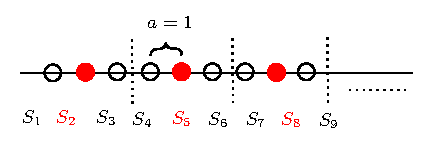
\includegraphics[width=0.6\textwidth]{../lessons/20_image/1.pdf}
\caption{\label{fig:20_1} Description.}
\end{figure}

Sum over the spins with the empty circle at the border of each clok, keeping the spins full circle untouched.
We obtain Figure \ref{fig:20_2}.

\begin{figure}[h!]
\centering
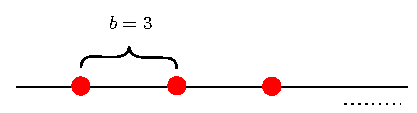
\includegraphics[width=0.6\textwidth]{../lessons/20_image/2.pdf}
\caption{\label{fig:20_2} Description.}
\end{figure}

Let us see how it works for the two blocks \( [S_1,S_2,S_3] \) and \( [S_4,S_5,S_6] \). Let us call
\begin{equation}
  S_2 \equiv S_1', \quad S_5 = S_2' \quad \text{fixed}
\end{equation}
\begin{equation}
  \sum_{S_3 = \pm 1}^{}   \sum_{S_4 = \pm 1}^{}  \exp [ k S_1' S_3 + k S_3 S_4 + k S_4 S_2']
\end{equation}
Since
\begin{equation}
  e^{k S_3 S_4}  = \cosh (k) ( 1 + x S_3 S_4)
\end{equation}
with
\begin{equation}
  x \equiv \tanh k
\end{equation}
we have
\begin{equation}
  \sum_{S_3,S_4}^{} \qty(\cosh k)^3 \qty(1 + x S_1' S_3) \qty(1 + x S_3 S_4) \qty(1 + x S_4 S_2')
\end{equation}
Performing the expansion and summing over \( S_3, S_4 \)  it is easy to show that (to do)
\begin{equation}
  Z_{N'}' (k') = \Tr_{ \{ S_I' \}  } \qty[ 2 ^{2N'} \qty( \cosh k)^{3N'} \qty(1 + x^3 S_I' S_{I+1} )  ]
  \label{eq:20_5}
\end{equation}
This must have the same form of \( Z_N (k) \). Hence, we should rewrite equation \eqref{eq:20_5} as
\begin{equation}
  Z_{N'}' (k') = \Tr_{ \{ S_I' \}  } \exp [ - \beta \mathcal{H}' (k')]
\end{equation}
with
\begin{equation}
  - \beta \mathcal{H}' = N' g (k,k') + k' \sum_{I}^{} S_I' S_{I+1}'
\end{equation}
We note that
\begin{equation}
\begin{split}
2^2 \qty(\cosh k)^3 (1 + x^3 S_I' S_{I+1}')   &=  2^2 \frac{\cosh k'}{\cosh k'}
 \qty(\cosh k)^3  (1 + x^3 S_I' S_{I+1}') \\
 & = 2^2 \frac{(\cosh k)^3}{\cosh k'}
  \qty(\cosh k')  (1 + x' S_I' S_{I+1}') \\
  & = 2^2 \frac{(\cosh k)^3}{\cosh k'}
   \exp (k' S_I' S_{I+1}') \\
   & = \exp [ 2 \ln{2} + \ln{ \qty[ \frac{(\cosh k)^3}{\cosh k'}] }  + k' S_I' S_{I+1}' ]
\end{split}
\end{equation}
It is ok with
\begin{equation}
  \begin{cases}
   g(k,k') = 2 \ln{2} +  \ln{ \qty[ \frac{(\cosh k)^3}{\cosh k'}] } \\
   x' = x^3  \iff k'= \tanh^{-1} \qty[ (\tanh k)^3] \Rightarrow k' = R_{b=3} (k)\\
   N' = \frac{N}{b}
  \end{cases}
\end{equation}
For \( x' = x^3 \), we have two fixed points
\begin{equation}
  \begin{cases}
   x^* = 0 \iff k \rightarrow 0 \iff T \rightarrow \infty \\
   x^* = 1^- \iff k \rightarrow \infty  \iff T \rightarrow 0
  \end{cases}
\end{equation}
For \( \forall x_0 < 1 \), we have \( R^{(n)} \overset{n \rightarrow \infty }{\longrightarrow} 0^+ \), \( x=1 \) is an unstable fixed point, as shown in Figure  \ref{fig:20_3}.
\begin{figure}[h!]
\centering
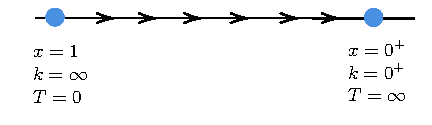
\includegraphics[width=0.6\textwidth]{../lessons/20_image/3.pdf}
\caption{\label{fig:20_3} Description.}
\end{figure}
We have
\begin{equation}
  \xi (x') = \frac{\xi (x)}{b}, \quad \text{with } x' = x^b
\end{equation}
where \( b \) is arbitrary. Let us choose \( b = c / \ln{x}  \):
\begin{equation}
  \xi (x^b) = \xi  \qty(e ^{b \ln{x} }) = \xi (e^c) = \frac{\xi (x)}{b}
  = \qty(\frac{c}{\ln{x} })^{-1} \xi (x)
\end{equation}
Finally,
\begin{equation}
  \xi (e^c) = \frac{\ln{x} }{c} \xi (x) \quad \Rightarrow \xi (x) = \frac{c \xi (e^c)}{\ln{x} } = \frac{const}{\ln{x} }
\end{equation}
\begin{equation}
  \xi (k) = \frac{const}{\ln{\qty(\tanh k) } }
\end{equation}
equal to the exact model in \( D=1 \).
\( k \rightarrow \infty  \) \( (x \rightarrow 1) \), we have
\begin{equation}
  \xi \sim e^{const/T}
\end{equation}
finite \( \forall k \neq \infty  \).

\section{Decimation procedure for \( D>1 \) (proliferation of interactions)}
Ioing on a square lattice, block transformation (length \( b \)). There are problems with the spins at the boundaries.
In order to get \( Z_{N'}' (k') = Z_N (k) \), at least an additional term in the Hamiltonian must be introduced
\begin{equation}
  \mathcal{H} \rightarrow \mathcal{H}' = \mathcal{H}' (k',k_2')
\end{equation}
This unfortunately occurs at each iteration! There is an uncontrolled proliferation and approximations are necessary.
\begin{example}{Decimation of Ising on square lattice}{}
  \( x \): spin to sum over
\begin{equation}
  \begin{cases}
   k' = \frac{1}{4} \ln{\cosh 4 k} \\
   L' = \frac{1}{8} \ln{\cosh 4 k} \\
   Q' = \frac{1}{8} \ln{\cosh 4 k} - \frac{1}{2} \ln{\cosh 2 k}\\
  \end{cases}
\end{equation}
(4 spins). The approximations are:
\begin{enumerate}
\item Neglect \( Q' \) term.
\item Omit explicit dependence on \( L' \). Hence, assuming \( k'+L' \rightarrow k' \). 1 recursion
\begin{equation}
  k' = \frac{3}{8} \ln{\cosh 4 k}
\end{equation}
\begin{equation}
  \begin{cases}
   k^{(n)} \overset{n \rightarrow \infty }{\longrightarrow} \infty  & k_0 > k_c \\
   k^{(n)} \overset{n \rightarrow \infty }{\longrightarrow} 0  & k_0 < k_c
  \end{cases}
\end{equation}
where \( \infty ,0 \) are stable fixed point.
\begin{equation}
  \delta k' = \lambda _t \delta k = l^{\lambda _t} \delta k
\end{equation}
where
\begin{equation}
  \lambda _t = \eval{\dv{k'}{k} }_{k=k_c}
\end{equation}
For \( l = \sqrt{2}  \),
\begin{equation}
\begin{split}
Y_t  &= \frac{\ln{\lambda _t} }{\ln{l} } = \frac{1}{\ln{\sqrt{2} } } \ln{\qty(\dv{k'}{k})_{k=k_c} }   \\
& = \frac{1}{\ln{\sqrt{2} } }  \ln{\qty(\dv{}{k} \qty(\frac{3}{8} \ln{(\cosh 4k)} ) ) } = 1.070
\end{split}
\end{equation}
we have also
\begin{equation}
  \nu = \frac{1}{Y_t} = 0.9345, \quad \alpha = 2 - \frac{d}{Y_t} = 0.1313
\end{equation}
\end{enumerate}

\end{example}








\end{document}
